\begin{figure}[t!]
    \vspace{-1mm}
    \centering
    \includegraphics[width=1\linewidth]{imgs/problem_formulation.png}
    \vspace{-6.5mm}
    \caption{\textbf{World State Formulation.} We approximate the intractable 4D world state $\mathcal{W}_t$ by decoupling it into two trackable representations: a temporally-invariant static 3D environment $\mathcal{M}_{static}$ via $T$-axis projection, and 2D video sequences of dynamic entities $\mathcal{M}_{dyn,t}$ via $Z$-axis projection.}
    \label{fig:problem_formulation}
    \vspace{-4.5mm}
\end{figure}

\vspace{-2.5mm}
\section{Methods}
\vspace{-1.5mm}

We propose \textcolor{blue}{\textbf{LiveWorld}}, a video world model framework designed to maintain and continuously evolve the out-of-sight dynamics of the currently unobserved world. Unlike previous video world models that follow an observer-centric paradigm---conflating world evolution with rendering and freezing out-of-view regions into static snapshots---our system explicitly decouples temporal evolution from spatial rendering. By implementing a monitor-centric pipeline, we autonomously model the temporal progression of active entities, narrowing the gap between the 2D video world modeling and the 4D dynamic world.



\vspace{-2.5mm}
\subsection{Problem Formulation}
\vspace{-1.5mm}
\subsubsection{Decoupling World Evolution from Observation Rendering.}
\label{sec:problem_formulation}
The world continues to evolve even when it is not observed. That is to say, an ideal world model should maintain a latent global world state $\mathcal{W}_{t}$ at each time step $t$, which specifies the underlying 4D scene at that moment. Since this state is view-independent, while an observed frame is only a camera-dependent projection, world modeling naturally decomposes into two processes: \textbf{(1) state evolution}, which updates the world over time, and \textbf{(2) rendering}, which maps the current state to an observation under a condition $C_t = \{C_t^{\text{cam}}, C_t^{\text{text}}\}$ (where $C_t^{\text{cam}}$ is the camera pose and $C_t^{\text{text}}$ is the semantic prompt). Formally,
\vspace{-1mm}
\begin{equation}
    \mathcal{W}_{t} = \mathcal{E}(\mathcal{W}_{<t}), \quad
    F_t = \mathcal{R}(\mathcal{W}_{t}, C_t).
    \label{eq:ideal_formulation}
\end{equation}
where $\mathcal{E}$ denotes the evolution engine and $\mathcal{R}$ denotes the conditioned renderer.

However, existing video world models do not maintain such an explicit world state. Instead, they compress the evolving 4D world into a history of 2D observations and directly predict the next frame from previously observed frames $\text{F}_{<t}=\left \{ F_{t-1}, F_{t-2},\dots ,F_0 \right \} $ and control signals $C_t$:
\begin{equation}
    F_t = \mathcal{V}_{\theta}(\text{F}_{<t}, C_t).
    \label{eq3:current_formulation}
\end{equation}

Under this formulation, world evolution and rendering are implicitly collapsed into a single black-box generator $\mathcal{V}_{\theta}$. The key limitation is that $\text{F}_{<t}$ contains only camera-dependent visual snapshots rather than the full underlying state $\mathcal{W}_{<t}$. In other words, the continuous 4D world is flattened into a sequence of 2D observations, and once a region leaves the field of view, the model has no explicit state to update, so its temporal progression is ignored and the region remain frozen at its last observed timestamp. We refer to this missing temporal progression as \textbf{out-of-sight dynamics}. 
% For example, if a dog is observed eating in $F_{t-k}$, the model stores only that observed appearance; when the camera revisits the same location at time $t$, it retrieves this outdated snapshot instead of reflecting the elapsed dynamics.


\subsubsection{Structured World-State Approximation}
To address this, \textbf{LiveWorld} restores an explicit separation between \textit{world evolution} and \textit{camera-conditioned rendering}. Directly maintaining a fully explicit 4D world state is impractical; therefore, we structurally approximate $\mathcal{W}_{t}$ based on a simple intuition: the static scene is temporally invariant, while temporal changes are concentrated in sparse dynamic entities.
Accordingly, we decompose the world state into two components as illustrated in Fig.~\ref{fig:problem_formulation}. \textbf{(1) Static background.} We collapse the time-invariant background of the world along the temporal axis into a static 3D scene representation $\mathcal{M}_{static}$. For \textbf{(2) dynamic entities}, their states continuously evolve over time. To maintain their up-to-date representations $\mathcal{M}_{dyn,t}$ (especially when they are out of the observer's sight), we introduce an explicit evolution function $G_{\theta}^{\text{evo}}$ serving as $\mathcal{E}$ in Eq.~\ref{eq:ideal_formulation}. It takes historical frames $\text{F}_{<t}$ containing active entities and simulates their continuous temporal progression, yielding the evolved dynamic representation at time $t$:
\vspace{-1mm}
\begin{equation}
    \mathcal{M}_{dyn,t} = G_{\theta}^{\text{evo}}(\text{F}_{<t})
    \label{eq4:dynamic_memory}
\end{equation}
\vspace{-1mm}
The up-to-date world state is then approximated as:
\begin{equation}
    \mathcal{W}_{t} \approx \{\mathcal{M}_{static}, \mathcal{M}_{dyn,t}\}
    \label{eq:world_state}
\end{equation}
Under this formulation, the video generator no longer implicitly handles hidden temporal evolution. Instead, it serves strictly as a state-aware renderer $G_{\theta}^{\text{render}}$ (serving as $\mathcal{R}$ in Eq.~\ref{eq:ideal_formulation}) that projects the composed world state under the control signal $C_t$:
\begin{equation}
    F_t = G_{\theta}^{\text{render}}(\mathcal{W}_{t}, C_t).
    \label{eq5:our_formulation}
\end{equation}

Implementing this decoupled formulation requires two components: (1) an explicit evolution mechanism $G_{\theta}^{\text{evo}}$ to update unobserved active regions over time (Sec.~\ref{sec:event_evolution}), and (2) a state-aware generative process $G_{\theta}^{\text{render}}$ that renders the composed 3D/2D world state into a coherent observation (Sec.~\ref{sec:observer_rendering}).




\vspace{-1mm}
\subsection{Unified State-Conditioned Video Backbone}
\label{sec:shared_video_backbone}
While the state-aware renderer $G_{\theta}^\text{render}$ and the evolution engine $G_{\theta}^\text{evo}$ are conceptually distinct, they share a fundamental generative paradigm: both synthesize future visual content conditioned on previous world states and external control signals. Motivated by this structural commonality, we propose a unified state-conditioned video diffusion model $G_{\theta}$ as an abstract interface model. Moreover, although we formulate state evolution at an atomic time step $t$ in Sec.~\ref{sec:problem_formulation}; In practice, we follow foundational video diffusion models\cite{wan, svd, hunyuanvideo} that generate video chunks in discrete autoregressive rounds. Therefore, we instantiate the generative step to cover a temporal window of $T$ frames. In the following sections, we use the notation $t:t+T$ to denote the generation of a $T$-frame sequence starting from timestamp $t$. Specifically, $G_{\theta}$ comprises a latent Video Diffusion Transformer (DiT)~\cite{wan} backbone, augmented with a dual-injection conditioning design to process explicit state projections and detailed appearances respectively:
% \noindent
% \vspace{-3mm}
\paragraph{Explicit state conditioning via state adapter.} To inject the maintained world states into the generation process, we employ a \textit{state adapter} initialized from \cite{vace}. This module functions as a ControlNet~\cite{controlnet}, taking a pixel-level projection tensor $\mathbf{P}_{t:t+T} \in \mathbb{R}^{T \times H \times W \times C}$ that represents the explicitly projected state for the target generation window. By injecting these signals into the DiT backbone, the state adapter imposes strict, explicit pixel-level guidance for the generated frames, ensuring consistency with the underlying world state.

% \noindent
% \vspace{-5mm}
\paragraph{Incorporating complementary appearance references.} Because the projected state $\mathbf{P}_{t:t+T}$ primarily serves as structural and positional guidance and may lack fine-grained visual details, inspired by \cite{iclora,spatia,catvton}, we register learnable LoRA parameters to the DiT backbone to accept concatenated historical reference frames. These references typically include a temporal anchor (e.g., the immediately preceding frames) to maintain motion continuity, and appearance anchors (retrieved from past frames) to fill in dense visual textures. We concatenate these reference frames along the token axis to the input of the DiT backbone. By flexibly configuring the input projection $\mathbf{P}_{t:t+T}$ and the appearance references, this unified backbone can be seamlessly instantiated for entirely different roles. As detailed below, we utilize this shared architecture to perform autonomous unobserved evolution (Sec.~\ref{sec:event_evolution}) and observer-centric spatial rendering (Sec.~\ref{sec:observer_rendering}).

\begin{tcolorbox}[width=1.0\linewidth, colframe=blackish, colback=lightgraybg, boxsep=0mm, arc=1mm, left=1mm, right=1mm, top=1mm, bottom=1mm]
\textbf{Unified Backbone Interface.} The shared architecture $G_{\theta}$ synthesizes a $T$-frame video chunk $V_{t:t+T}$, guided by three abstract conditioning inputs: an explicit state projection $\mathbf{P}$ (which encapsulates the geometric camera control $C^{\text{cam}}$), supplementary appearance references $\mathbf{A}$, and the text prompt $C^{\text{text}}$.
\begin{equation}
    V_{t:t+T} = G_{\theta}(\mathbf{P}_{t:t+T},\, \mathbf{A},\, C_{t:t+T}^{\text{text}})
    \label{eq:interface}
\end{equation}
\end{tcolorbox}


\begin{figure}[t]
    \centering
    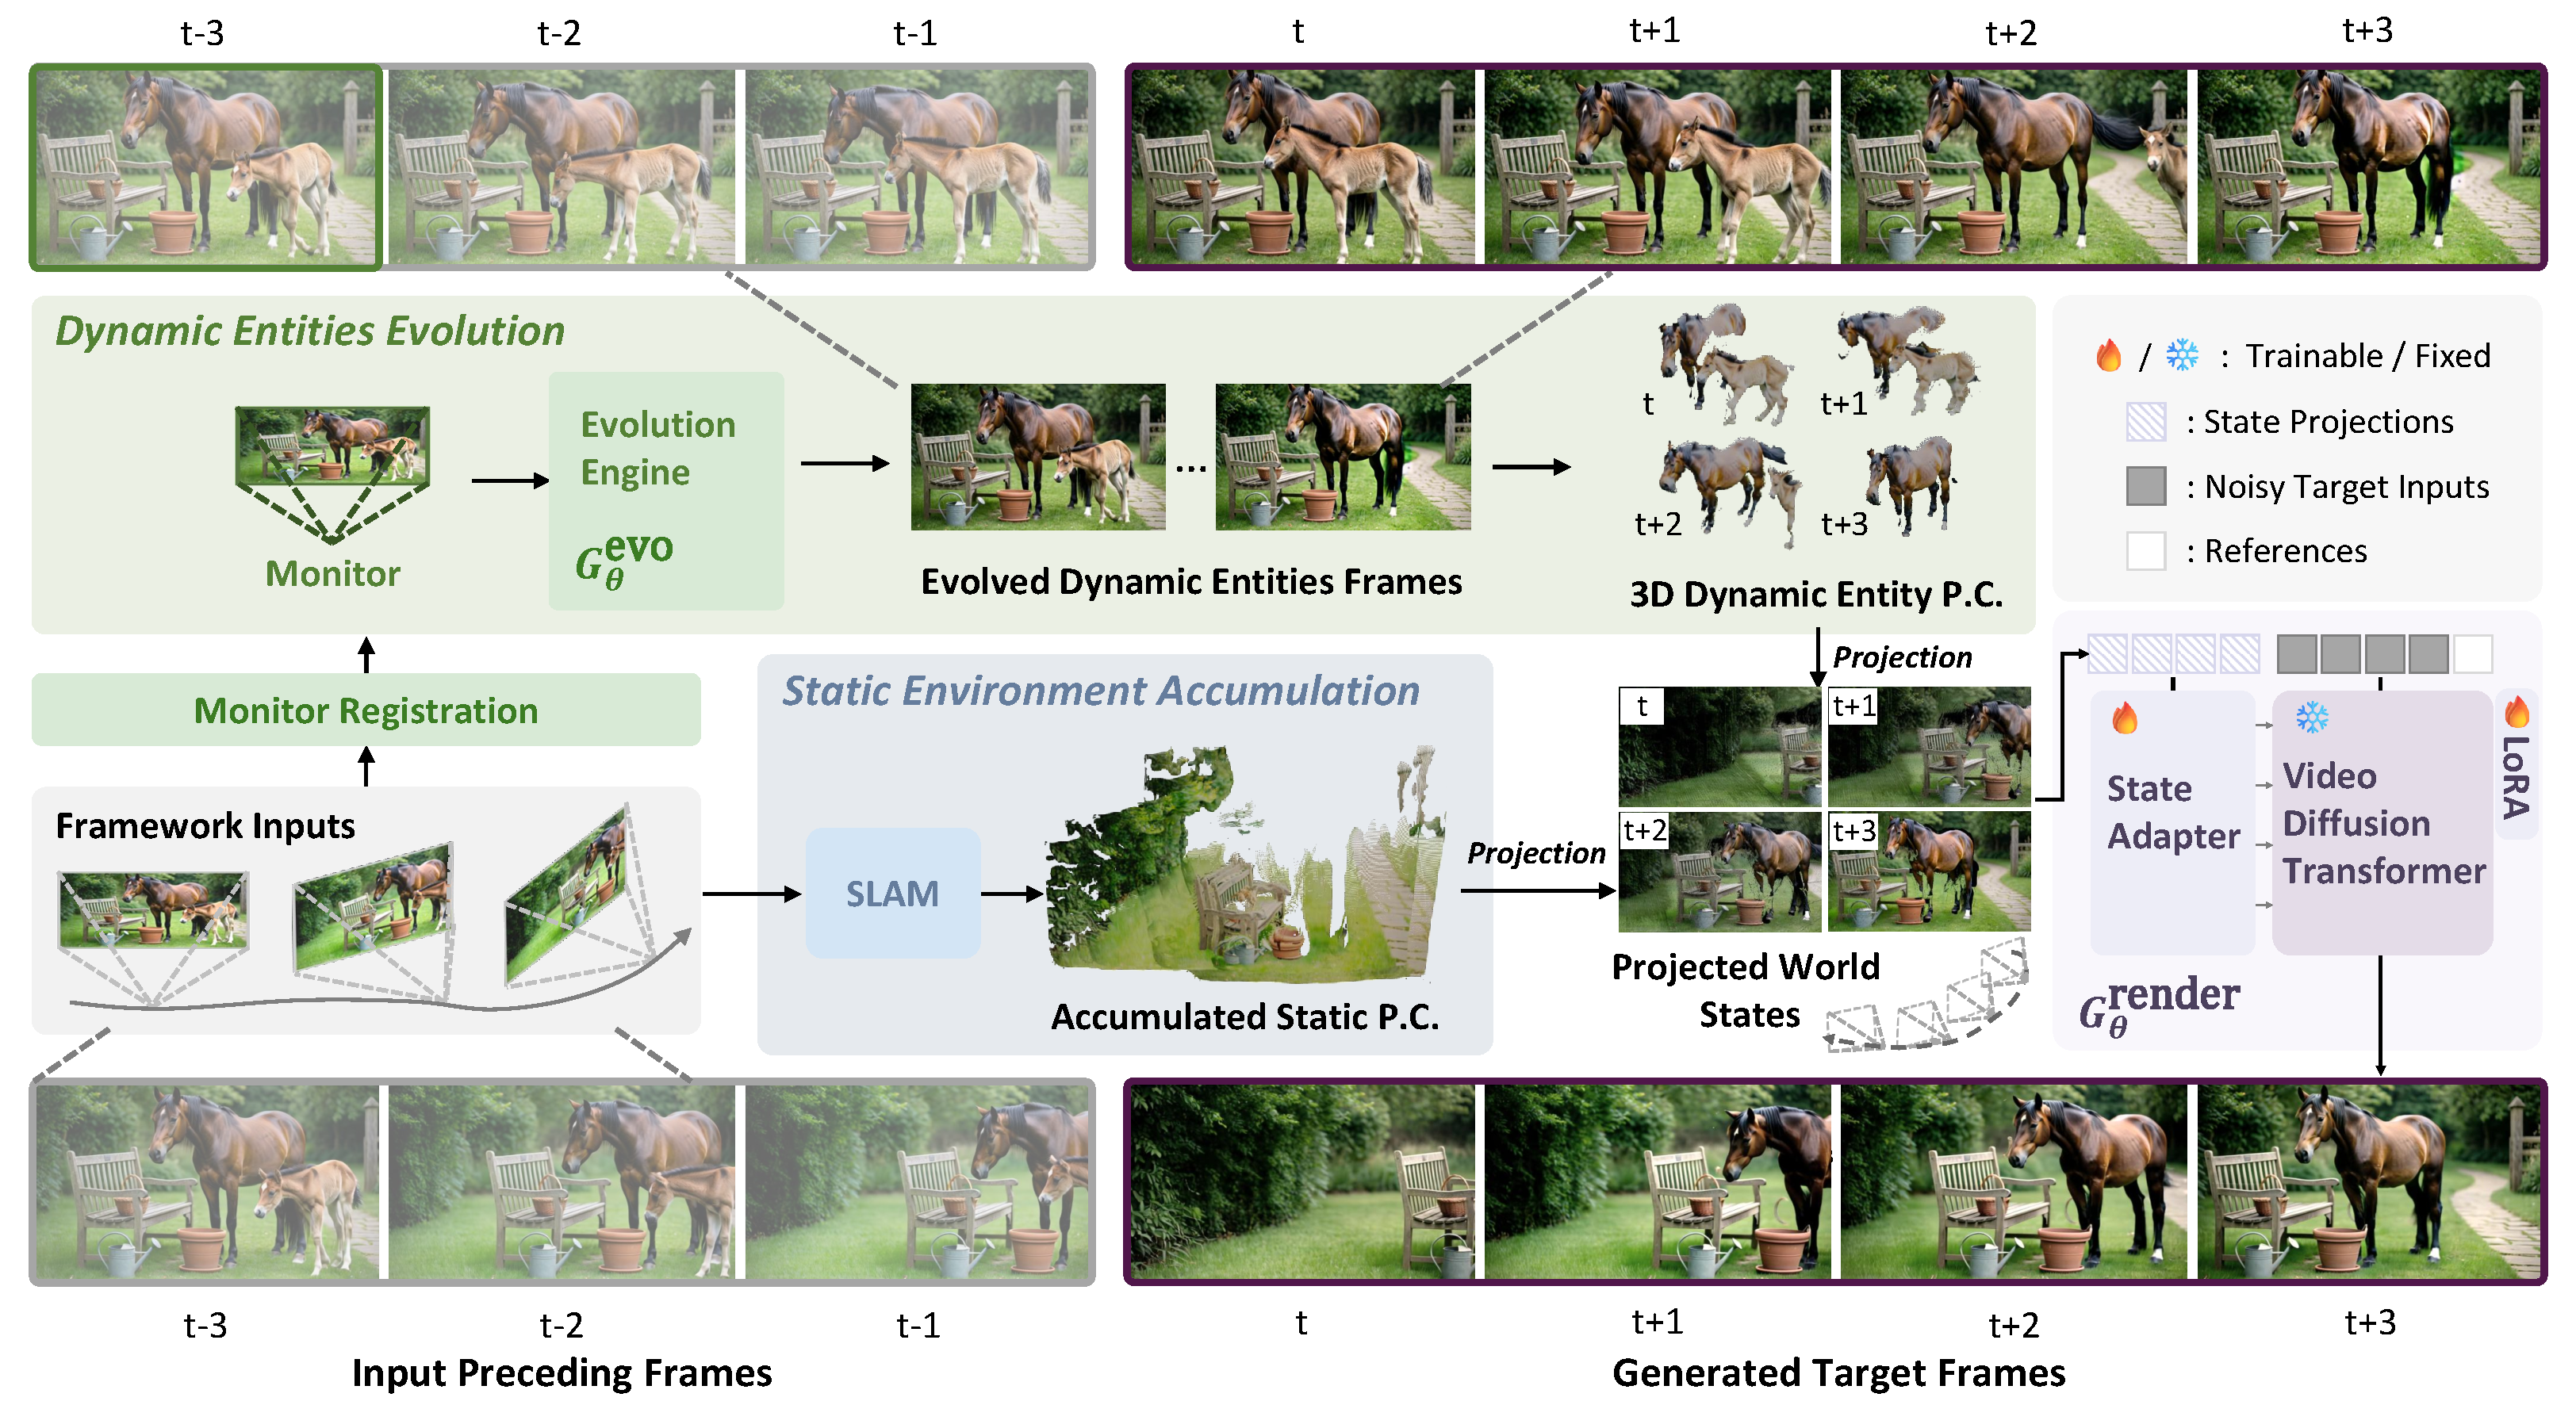
\includegraphics[width=1\linewidth]{imgs/main.pdf}
    \vspace{-4.5mm}
    \caption{\textbf{LiveWorld overview.} Our system explicitly decouples world modeling into two processes. \textbf{(1) Static Accumulation (Blue):} Temporally-invariant backgrounds are fused into a static 3D point cloud via SLAM. \textbf{(2) Dynamic Evolution (Green):} Stationary monitors use the Evolution Engine $G_{\theta}^{\text{evo}}$ to fast-forward the out-of-sight progression of active entities, lifting them into 4D point clouds. \textbf{(3) State-aware Rendering (Purple):} Both representations are projected onto the target camera trajectory. This geometric projection, alongside appearance references, guides the renderer $G_{\theta}^{\text{render}}$ to synthesize coherent observations reflecting the elapsed dynamics.}
    \label{fig:main}
    \vspace{-2.5mm}
\end{figure}

\begin{figure}[t]
    \centering
    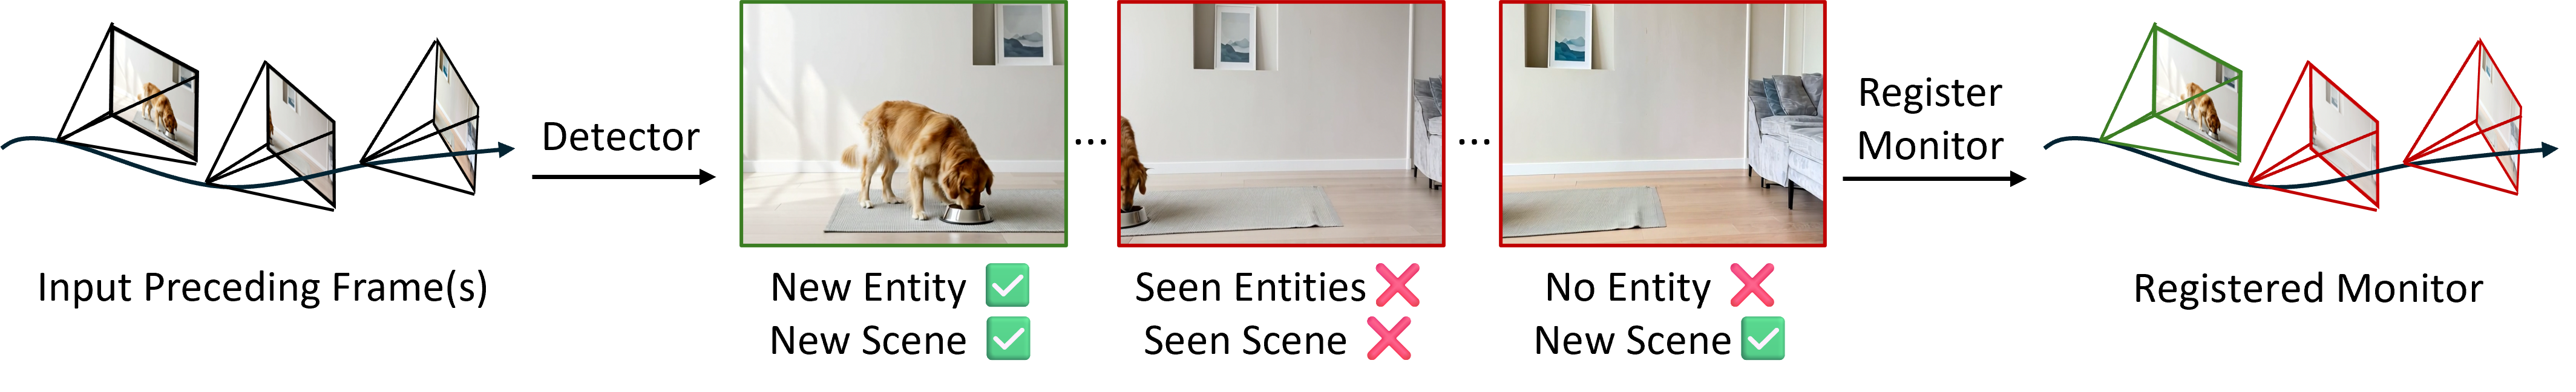
\includegraphics[width=1\linewidth]{imgs/registration.png}
    \vspace{-7mm}
    \caption{Given one or multiple preceding frames from the previous round, we first detect if the scene visited by the observer contains active dynamic entities, using off-the-shelf VLMs and segmentors. Following a positive detection, we further validate if the entity and scene are already registered by existing monitors.}
    \label{fig:monitor_registration}
    \vspace{-4mm}
\end{figure}

\vspace{-1mm}
\subsection{Evolving World States}
In this section, we introduce the maintenance of the world state formulated in Eq.~\ref{eq:world_state} through a continuous, multi-round update process. In each generation round spanning the temporal window $t$ to $t+T$, the system iteratively prepares the up-to-date world state $\mathcal{W}_{t:t+T}$ by executing two fundamental updates: \textbf{(1)} accumulating newly observed static regions into the temporally-invariant 3D representation $\mathcal{M}_{static}$, and \textbf{(2)} autonomously updating the registered active entities via the evolution function $G_{\theta}^\text{evo}$ to simulate their out-of-sight dynamics over this window into $\mathcal{M}_{dyn,t:t+T}$.
\vspace{-5mm}
\subsubsection{Accumulating the static environment $\mathcal{M}_{static}$}
We represent the static environment $\mathcal{M}_{static}$ as an accumulated background point cloud. For each historically observed frame in $\text{F}_{<t}$, the background is segmented~\cite{sam3} and incrementally fused into a global static point cloud via a feed-forward SLAM framework Stream3R~\cite{stream3r2025}, enabling continuous online memory accumulation.

\vspace{-3mm}
\subsubsection{Evolving dynamic entities $\mathcal{M}_{dyn}$}
\label{sec:event_evolution}
We implement the evolution function $\mathcal{E}$ through a \textit{monitor-driven dynamic evolution} system. Instead of modeling the entire unobserved world, we dynamically allocate stationary virtual agents, termed \textit{Monitors}, to track localized active regions.

% \noindent
\vspace{-2mm}
\paragraph{Defining and registering monitors.} Monitors are a set of generative agents placed at different world positions along the past camera trajectory, aiming to continuously evolve the previously observed scenes containing dynamic entities. They are powered by shared modules: a VLM-based detector~\cite{qwen3vl, sam3} for entity detection, and the evolution engine $G_{\theta}^\text{evo}$.
Specifically, as illustrated in Fig.~\ref{fig:monitor_registration}, before generating the new chunk $F_{t:t+T}$, we inspect the previously generated frames $F_{t-T:t}$ using the detector. If an unseen dynamic entity is detected along the observer's trajectory, and its spatial overlap with existing monitored regions falls below a certain threshold, a new monitor is registered at that specific pose (denoted as its \textit{anchor pose}). The monitor then takes the observed frame as its \textit{anchor frame}. To maintain computational efficiency, we limit the number of active monitors to $M$, discarding the one farthest from the observer when this limit is exceeded.

\vspace{-2mm}
% \noindent
\paragraph{Monitor-driven dynamic evolution.} After registration, we take the instantiated evolution engine $G_{\theta}^\text{evo}$ to simulate ongoing out-of-sight dynamics in the upcoming round for each monitor. First, to fix the monitor at the desired position without camera movements, recalling the state injection formulation (Eq.~\ref{eq:interface}), 
% we instantiate $G_{\theta}^\text{evo}$'s explicit state condition $\mathbf{P}_{t:t+T}$ with the repeated background of the anchor frame to be $\mathbf{P}^{\text{bg}_{anc}}_{t:t+T}$, simulating a static scene state with no background pixel change, forcing $G_{\theta}^\text{evo}$ to generated frames with static background. Second, to evolve foreground entities, we condition  $G_{\theta}^\text{evo}$ on text prompts $C_{t:t+T}^{text}$ detailing anticipated entity actions. For the supplementary appearance references, we cropped entities $\mathbf{A}^{\text{entity}}$ from the anchor frame and feed them into the DiT backbone. Passing these inputs through the shared backbone yields a synthesized local video of the entity's continued dynamics over the $t:t+T$ window.
We instantiate the explicit state condition $\mathbf{P}_{t:t+T}$ of $G_{\theta}^{\text{evo}}$ using the static background from the anchor frame, and condition $G_{\theta}^\text{evo}$ on text prompts $C_{t:t+T}^{text}$ detailing the anticipated actions of the entities to evolve the foreground entities, then cropped entities $\mathbf{A}^{\text{entity}}$ from the anchor frame for the additional appearance references. These inputs are processed through $G_{\theta}^{\text{evo}}$ to generate a local video depicting the continued dynamics of the entity over the interval $t:t+T$.

% \noindent
\vspace{-2mm}
\paragraph{Asynchronous temporal synchronization.} Since a new entity may emerge mid-round (e.g., first observed by the main camera at $t_a \in (t-T, t)$), its initial state is asynchronous with the current global timestamp $t$. To synchronize it before the next evolution round, the evolution engine $G_{\theta}^{\text{evo}}$ first synthesizes the missing local frames from $t_a$ to $t$. This aligns the entity's state with the global timeline, preparing it for the upcoming $t:t+T$ evolution.


\begin{tcolorbox}[width=1.0\linewidth, colframe=blackish, colback=lightgraybg, boxsep=0mm, arc=1mm, left=1mm, right=1mm, top=1mm, bottom=1mm]
\textbf{Instantiation I: Evolution Engine ($G_{\theta}^{\text{evo}}$).} We instantiate $G_{\theta}$ to synthesize the monitor's local video $v_{t:t+T}^{\text{monitor}}$, which is subsequently lifted to form $\mathcal{M}_{dyn, t:t+T}$. The inputs are specialized for localized event evolution:
\begin{equation}
    v_{t:t+T}^{\text{monitor}} = G_{\theta}^{\text{evo}}(\mathbf{P}^{\text{bg}_{anc}}_{t:t+T},\, \mathbf{A}^{\text{entity}},\, C_{t:t+T}^{\text{text}})
\end{equation}
where $\mathbf{P}^{\text{bg}_{anc}}_{t:t+T}$ is the repeated static anchor frame background, $\mathbf{A}^{\text{entity}}$ is the cropped entity reference, and $C_{t:t+T}^{\text{text}}$ is the action prompt.
\end{tcolorbox}

% \noindent
\vspace{-2.5mm}
\paragraph{Integrating dynamic memory.} Finally, equipped with the known monitor anchor pose and per-frame depth, the monitor unprojects the 2D dynamic foreground from $v_{t:t+T}^{\text{monitor}}$ back into the 3D world space. This lifting process yields a localized, temporally evolving 4D Monitor Point Cloud. This explicit 4D representation constitutes the concrete output $\mathcal{M}_{dyn, t:t+T}$ defined in Eq.~\ref{eq4:dynamic_memory}, providing the up-to-date dynamic memory to compose $\mathcal{W}_{t:t+T}$.

\vspace{-3mm}
\subsection{Rendering World States}
\vspace{-0.5mm}
\label{sec:observer_rendering}
With the updated world state $\mathcal{W}_{t:t+T}$ prepared (including the static point cloud $\mathcal{M}_{static}$ and the evolved $\mathcal{M}_{dyn, t:t+T}$), the final step is to synthesize the observer's visual experience. Here, we instantiate the unified backbone $G_{\theta}$ (Sec.~\ref{sec:shared_video_backbone}) into its second role: the state-aware renderer $G_{\theta}^\text{render}$. 

Unlike the evolution engine that operates on stationary monitor poses, $G_{\theta}^\text{render}$ synthesizes the scene from a continuously moving observer trajectory. Specifically, we project both the static 3D environment and the evolved dynamic monitor frames into the observer's novel camera views to construct the global state projection $\mathbf{P}_{t:t+T}$. Guided by this projection and historical reference frames, $G_{\theta}^\text{render}$ autoregressively renders the final observation video $F_{t:t+T}$, completing the generation loop.
\vspace{-3mm}
\subsubsection{Projecting the evolved world states}
% At each generation round spanning $t$ to $t+T$, the updated static point cloud $\mathcal{M}_{static}$ and the evolved dynamic 4D point clouds $\mathcal{M}_{dyn, t:t+T}$ are used to derive the explicit state projection $\textbf{P}_{t:t+T}$ for the state adapter. 
% Specifically, recalling the unified backbone configuration (Sec.~\ref{sec:shared_video_backbone}), to instantiate the renderer $G_{\theta}^{\text{render}}$ for generating the observation chunk $F_{t:t+T}$ under the camera trajectory $C_{t:t+T}^{\text{cam}}$, we project the composed world state $\mathcal{W}_{t:t+T} \approx \{\mathcal{M}_{static}, \mathcal{M}_{dyn, t:t+T}\}$ onto the target sequence of views:
At each generation round spanning $t$ to $t+T$, the updated static point cloud $\mathcal{M}_{static}$ and the evolved dynamic 4D point clouds $\mathcal{M}_{dyn, t:t+T}$ are used to derive the explicit state projection $\textbf{P}_{t:t+T}$ for the state adapter of $G_{\theta}^{\text{render}}$:
\vspace{-1mm}
\begin{equation}
    \mathbf{P}_{t:t+T} = \text{Proj}(\{\mathcal{M}_{static}, \mathcal{M}_{dyn, t:t+T}\}, C_{t:t+T}^{cam}) \in \mathbb{R}^{T \times H \times W \times C}
\end{equation}
As a result, generation strictly conditioned on the state projection $\mathbf{P}_{t:t+T}$ enables explicit camera control while consistently reflecting the spatial evolution of both the static environment and dynamic events throughout the sequence.

\vspace{-3mm}
\subsubsection{Reference frames retrieval for appearance guidance}
% To complete the rendering process, $G_{\theta}^{\text{render}}$ supplements the sparse geometric projection $\mathbf{P}_{t:t+T}$ with dense visual details via the Appearance LoRA. We retrieve the latest preceding frame $F_{t-1}$ as a temporal anchor for motion continuity and support image-to-video generation. Additionally, if $C_{t:t+T}^{cam}$ revisits previously explored regions, we retrieve the corresponding historical frames from $\text{F}_{<t}$ as appearance anchors. This strategy ensures high visual fidelity and texture consistency across continuous explorations.
To supplement dense visual details through the registered LoRA of $G_{\theta}^{\text{render}}$, we retrieve the latest preceding frame $F_{t-1}$ as a temporal anchor for motion continuity and if $C_{t:t+T}^{cam}$ revisits previously explored regions, we retrieve the corresponding eariliest historical frames, containing least visual drifting, from $\text{F}_{<t}$ as appearance anchors. This strategy ensures high visual fidelity and texture consistency across continuous explorations.

\begin{tcolorbox}[width=1.0\linewidth, colframe=blackish, colback=lightgraybg, boxsep=0mm, arc=1mm, left=1mm, right=1mm, top=1mm, bottom=1mm]
\textbf{Instantiation II: Observer Renderer ($G_{\theta}^{\text{render}}$).} We instantiate $G_{\theta}$ to render the global observation chunk $F_{t:t+T}$ based on the composed world state and the text control:
\vspace{-1mm}
\begin{equation}
    F_{t:t+T} = G_{\theta}^{\text{render}}(\mathbf{P}_{t:t+T}^{\text{global}},\, \mathbf{A}^{\text{history}},\, C_{t:t+T}^{\text{text}})
\end{equation}
where $\mathbf{P}_{t:t+T}^{\text{global}} = \text{Proj}(\{\mathcal{M}_{static}, \mathcal{M}_{dyn, t:t+T}\}, C_{t:t+T}^{\text{cam}})$ integrates both static and out-of-sight dynamics, and $\mathbf{A}^{\text{history}}$ provides retrieved spatial textures.
\end{tcolorbox}


\vspace{-3mm}
\subsection{Model Training}
\label{sec:training}

The unified backbone $G_{\theta}$ is trained with the flow matching objective~\cite{sd3}. Given a clean target latent $\mathbf{z}_0$ encoded by a frozen VAE, noise $\boldsymbol{\epsilon} \sim \mathcal{N}(0, \mathbf{I})$, and timestep $t \sim \mathcal{U}[0,1]$, the training loss is:
\vspace{-0.5mm}
\begin{equation}
    \mathcal{L} = \mathbb{E}_{\mathbf{z}_0, \boldsymbol{\epsilon}, t} \left\| \mathbf{v}_\theta(\mathbf{z}_t, t, \mathbf{P}, \mathbf{A}, C) - (\boldsymbol{\epsilon} - \mathbf{z}_0) \right\|^2
\end{equation}
where $\mathbf{z}_t = (1-t)\mathbf{z}_0 + t\boldsymbol{\epsilon}$. The loss is computed only on target frames; preceding and reference frames serve as clean conditioning tokens. We adopt a two-stage strategy: \textbf{Stage 1} trains the state adapter with the backbone frozen, and \textbf{Stage 2} freezes the adapter and fine-tunes LoRA modules on the backbone's attention layers for appearance reference integration. All encoders remain frozen throughout. Training data construction can be found in the Appendix.